% --- PRÉAMBULE ---
\documentclass[a4paper, 11pt]{article}

% --- Paquets pour le français et l'encodage ---
\usepackage[utf8]{inputenc}
\usepackage[T1]{fontenc}
\usepackage[french]{babel}

% --- PAQUETS CORRIGÉS/AJOUTÉS ---
\usepackage{xcolor} % Pour définir et utiliser des couleurs
\usepackage{colortbl} % Pour la commande \rowcolor dans les tableaux
\usepackage{tabularx} % Pour l'environnement tabularx
\usepackage{enumitem} % Pour personnaliser les listes (label=$\circ$ et label=$\bullet$)
\usepackage{array}    % Pour améliorer les tableaux

\usepackage{geometry}
\geometry{a4paper, margin=2.5cm} % Marges
\usepackage{graphicx} % Pour inclure des images
\usepackage{hyperref} % Pour les liens cliquables (ex : table des matières)
\usepackage{xurl}
\hypersetup{
    colorlinks=true,
    linkcolor=black,
    urlcolor=blue,
}
\usepackage{amsmath} % Pour les formules mathématiques
\usepackage{appendix}
\usepackage{pdfpages}
\usepackage{makecell}
\usepackage{ragged2e}

% --- Coloration / code ---
\usepackage{listings}
\lstdefinelanguage{Chips}{
  morekeywords={logical, physical,object,system,init,then,spread,collect,as,with,implementation,input,stop,among,ctx,using,actuator,sensor},
  sensitive=true,
  morecomment=[l]{//},
  morestring=[b]"
}
\lstset{
  basicstyle=\ttfamily\small,
  keywordstyle=\color{blue}\bfseries,
  commentstyle=\color{gray},
  stringstyle=\color{red!60!black},
  showstringspaces=false,
  columns=fullflexible,
  frame=single,
  breaklines=true
}
\DeclareRobustCommand{\prog}[1]{\begingroup\urlstyle{tt}\nolinkurl{#1}\endgroup}
\newcommand{\kw}[1]{\textbf{#1}}


% --- DÉBUT DU DOCUMENT ---
\begin{document}

\justifying


\begin{titlepage}
  \begin{center}
    
\begin{figure}[ht]
    \centering
    \begin{minipage}{0.45\textwidth}
        \centering
        
\includegraphics[height=22mm]{logo-UFRST-DeptInfo.png}
    \end{minipage}
    \hfill % Petit espacement entre les deux blocs
    \begin{minipage}{0.45\textwidth}
        \centering
        
\includegraphics[height=22mm]{LOGO_UMLP.png}
    \end{minipage}
\end{figure}
    
   \vspace{1cm}
% \marginpar{OlgaK : les logos UMLP et UFR ST doivent être ensemble en haut, en plus petit}   

         % --- Université et Master ---
  {\large\scshape Université Marie \& Louis Pasteur \\ Département informatique\par} % \scshape pour petites majuscules
  \vspace{0.5em} % Petit espace
  {\large Master 2 en Ingénierie Système et Logiciel\par} % Taille de police standard pour le master
    
        \vspace{1.2cm}
    \centerline{\hbox to 13cm{\hrulefill}}
    \vspace{0.3cm}
    {\sc \Large  \uppercase{{
        Implantation d'un parseur et ajout d'un jeu d'instructions pour le langage CHIPS
    }}}
    \centerline{\hbox to 13cm{\hrulefill}}
    
    \vspace{1.2cm}
    {\sc \Large {DOLARD ANTON} \\ [0.5 cm]
    \sc \Large {FOCHEUX VITAL} \\ [0.5 cm]
    \sc \Large {GAUTHIER JULIEN}\\ [0.5 cm]
    \sc \Large {TUTRICES :} \\ [0.5 cm]
    \sc \Large {GALLONE ANNA} \\ [0.5 cm]
    \sc \Large {KOUCHNARENKO OLGA}\\ [0.5 cm]
    }
    \vspace{1.5cm}

    \begin{figure}[h]
		\centering
		
\includegraphics[width=0.48\textwidth]{CHIPS.png}
    \end{figure}
    
    \vspace{0.5cm}
    

    
    \hbox to \textwidth{\hrulefill}
    \vspace{0.2cm}
    {\sc  RAPPORT DE PROJET DE MASTER 2 INGÉNIERIE SYSTÈME ET LOGICIEL - ANNÉE 2025/2026}
    
  \end{center}
\end{titlepage}



\thispagestyle{empty}
\clearpage

\newpage

\section*{Remerciements}

Nous tenons à remercier nos tutrices de projet, Mme \textsc{KOUCHNARENKO} et Mme \textsc{GALLONE} 
qui ont su nous conseiller tout au long de ce projet.

\newpage

\newpage
\tableofcontents % Crée la table des matières
\newpage

\newpage
\setcounter{page}{1} % Commence la numérotation des pages à 1 ici

\section{Introduction}

% Chips est un langage de programmation conçu par Mme \textsc{GALLONE} au cours de sa thèse. Il a pour objectif d'être compilé vers le langage BIP.

Dans le cadre de la modélisation de systèmes distribués en vue de leur simulation et implantation, un langage est en cours de développement au DISC\footnote{Département Informatique de Systèmes Complexes}. Ce langage, CHIPS\footnote{Control of Hierarchical Interconnected Programmable Systems}, vise à représenter les applications distribuées sous la forme de deux graphes : \textbf{un graphe fonctionnel} représentant les algorithmes par ses nœuds et des flux de données par ses arêtes, et \textbf{un graphe de dépendance physique} utilisant les mêmes nœuds et ajoutant un second type d'arêtes pour signifier le rattachement des algorithmes à leur support physique. \\
%TODO revoir cette intro
Lors de ce rapport, nous allons détailler les différents aspects conceptuels et techniques de ce projet. Nous commencerons par présenter les besoins et objectifs du projet dans la section \ref{sec:besoins_objectifs}. Ensuite, nous détaillerons les algorithmes et les technologies utilisés et mis en place pour mettre en oeuvre de projet dans la section \ref{sec:algorithmes_techno}. Comme le lexing et parsing de la grammaire mais aussi la sérialisation vers le langage XMI\footnote{XML Metadata Interchange}. Suivi des explications pour gérer les erreurs au moyen de génération de tests ainsi que du parcours de l'AST\footnote{Abstract Syntax Tree} dans la section \ref{sec:verification_conformite}. Nous évoquerons une partie sur la gestion du projet et ce qui a été mis en oeuvre dans la section \ref{sec:gestion}. Enfin nous pourrons conclure ce projet sur un bilan technique où nous évoquerons ce qui a pu être réalisé mais aussi ce qui aurait pu être réalisé, et aussi un bilan personnel.


\section{Besoins et objectifs du projet}
\label{sec:besoins_objectifs}

\subsection{Contexte}
Le langage CHIPS s’inscrit dans une démarche de modélisation formelle des systèmes distribués. Il permet de décrire des architectures complexes en représentant explicitement les composants logiciels, leurs interconnexions et leurs supports physiques.

Toutefois, le langage CHIPS est encore en cours d'évolution et reste sujet à de futures modifications. Certaines constructions syntaxiques ne sont pas entièrement prises en charge par l'outil de compilation associé. Il est donc apparu nécessaire d'améliorer l'analyseur syntaxique existant afin de garantir une prise en charge complète et cohérente du langage.

Ce projet s’inscrit ainsi dans la continuité des travaux menés au DISC et contribue à l’évolution et à la stabilisation du langage CHIPS.

\subsection{Motivations}
La modélisation des systèmes distribués présente plusieurs avantages. Elle permet de concevoir une architecture de manière abstraite avant son implantation réelle. Cette approche réduit les coûts de développement et limite les erreurs en phase d’intégration. Les incohérences peuvent être détectées plus tôt, ce qui améliore la fiabilité globale du système.

La modélisation favorise également la modularité. Les composants sont décrits indépendamment de leur support d’exécution, ce qui facilite leur réutilisation et leur évolution. Elle ouvre aussi la voie à l’automatisation, notamment pour la génération de code, la transformation de modèles ou la production automatique de tests.

Dans ce contexte, l’amélioration du langage CHIPS et de ses outils constitue un enjeu important. Un langage plus robuste et mieux outillé permet de produire des modèles plus fiables, plus exploitables et plus facilement intégrables dans une chaîne de transformation et d’analyse.

\newpage
\subsection{Objectifs}

Parmi les objectifs, il y a ceux qui avaient été demandés, comme :
\begin{itemize}
    \item Compléter un parseur C++/Yacc/Bison.
    \item Intégrer de nouvelles constructions syntaxiques représentant les fonctions collectives\footnote{C'est fonctions sont collect et spread} qui n'étaient pas encore supportées par le langage.
    \item La gestion des erreurs syntaxiques et sémantiques.
\end{itemize} 


Mais certains objectifs ont pu être ajoutés au cours du projet, que cela soit par nos tutrices ou bien par nous, comme :
\begin{itemize}
    \item La sérialisation de l'AST vers le langage XMI.
    \item un modèle GBT\footnote{Grammar Based Testing} afin de créer des tests d'acceptation pour le langage.
\end{itemize}

\section{Algorithmes et technologies}
\label{sec:algorithmes_techno}

Cette partie est consacrée à la présentation des différents algorithmes et technologies employés dans le cadre de ce projet.

Pour le lexer et le parser du langage, nous avons opté pour \kw{Flex} et \kw{Yacc} en \prog{C++}. Ce choix a été motivé par notre familiarité antérieure avec ces outils, ainsi que par l'existence de ressources et d'exemples qui ont simplifié notre démarche.

Dans un second temps, nous aborderons la sérialisation de l'AST (Abstract Syntax Tree) vers le langage XMI. Dans un second temps, nous aborderons la sérialisation de l'AST (Abstract Syntax Tree) vers le langage XMI. \kw{XMI} (XML Metadata Interchange) est un standard créé par l'Object Management Group (\kw{OMG}) pour l'échange de métadonnées UML, basé sur XML. \footnote{Source : \url{https://fr.wikipedia.org/wiki/XML_Metadata_Interchang}}

\subsection{Lexing et parsing de la grammaire}

% Dans les deux prochaines sections, les figures citées se retrouveront dans la section \ref{sec:figures}.

\subsubsection{Lexing}

Afin d'avoir une grammaire utilisable, il faut que l’on puisse créer des jetons et des symboles terminaux. Pour cela, nous avons utilisé l'outil libre \kw{Flex} qui est un analyseur lexical. Il va nous permettre, grâce à des expressions régulières, de déterminer certains jetons comme :
\begin{itemize}
    \item \prog{DIGIT [0-9]} $\longrightarrow$ représentation d'un chiffre
    \item \prog{IDENT [a-zA-Z] [a-zA-Z0-9\_]*} $\longrightarrow$ représentation des identifiants
\end{itemize}

Ce qui nous permet par la suite de faire la représentation des littéraux (cf. figure \ref{fig:jetons_literal}), des opérateurs binaires et unaires (cf. figure \ref{fig:jetons_binaires_unaires}), des types de données et fonctions (cf. figure \ref{fig:jetons_type_donnees} et figure \ref{fig:jetons_type_func}), des littéraux qu'on peut retrouver dans d'autres langages comme C (cf. figure \ref{fig:jetons_C}) et enfin les littéraux qui sont spécifiques à CHIPS (cf. figure \ref{lst:jetons}).

Une fois tous les jetons terminaux instanciés, nous allons pouvoir nous en servir durant le parsing et la création de l'AST avec les règles de la grammaire que nous allons évoquer dans la partie suivante.

\newpage
\subsubsection{Parsing}

Une fois tous les jetons terminaux définis, nous allons pouvoir écrire les règles du langage, c'est ce qui nous permet, en parcourant la première règle, d'atteindre des règles "terminales" \footnote{C'est-à-dire qu'elle contient que des jetons terminaux ou bien les jetons non terminaux sont soit vides soit un seul jeton terminal}. Pour cela, nous utilisons l'outil \kw{Yacc} qui est un outil de génération d'analyseurs syntaxiques en langage \prog{C}.

\begin{lstlisting}[language=C, caption={Exemple de règle de la grammaire}, label={lst:grammar_physical}]
p_function_def:
    PHYSICAL_KW IDENTIFIER L_PARENTH pdf_parameter_list R_PARENTH
    with_section
    init_section
    then_section
    p_named_outputs { $$ = std::move(std::make_unique<physical_function_definition_node>(std::move($2), std::move($4), std::move($6), std::move($7), std::move($8), std::move($9))); 
                      $$->set_line(@$.bein.line); 
                      $$->set_column(@$.begin.column);}
    ;
\end{lstlisting}

Par exemple la règle pour définir une fonction physique (cf. Listing \ref{lst:grammar_physical}) où on va définir le nom de la règle, ici p\_function\_def, et on va lui définir la suite de jetons qu'elle peut prendre, ici des jetons terminaux qui sont : 
\begin{itemize}
    \item \prog{PHYSICAL\_KW} $\longrightarrow$ qui correspond au jeton \prog{physical}
    \item \prog{IDENTIFIER} $\longrightarrow$ qui correspond au jeton pour les identifiants
    \item \prog{L\_PARENTH} $\longrightarrow$ qui correspond au jeton pour \prog{(}
    \item \prog{R\_PARENTH} $\longrightarrow$ qui correspond au jeton pour \prog{)}
\end{itemize}

et des jetons non terminaux qui sont :
\begin{itemize}
    \item \prog{pdf\_parameter\_list} $\longrightarrow$ qui correspond à la règle de la grammaire pour la liste des paramètres des fonctions physiques
    \item \prog{with\_section} $\longrightarrow$ qui correspond à la règle de la grammaire pour la section \prog{with}
    \item \prog{init\_section} $\longrightarrow$ qui correspond à la règle de la grammaire pour la section \prog{init}
    \item \prog{then\_section} $\longrightarrow$ qui correspond à la règle de la grammaire pour la section \prog{then}
    \item \prog{p\_named\_outputs} $\longrightarrow$ qui correspond à la règle de la grammaire pour les outputs de la fonction physique
\end{itemize}

Après la définition de ou des règle(s), on va pouvoir créer le nœud de l'AST, où \$\$ correspond au nœud de l'AST sur lequel on va pouvoir potentiellement effectuer les fonctions de la classe. Le constructeur du noeud prend en paramètre \$X où X correspond au numéro du jeton dans la règle. Le constructeur prend presque toujours en paramètre des jetons non terminaux, seuls les jetons terminaux qui correspondent aux littéraux comme les identifiants, les booléens et les nombres peuvent être pris en paramètre. Dans cet exemple, l'identifiant de la fonction, qui est un jeton terminal, est pris en paramètre et il correspond à \$2.

Une fois le nœud instancié, nous allons pour certains nœuds utiliser leurs fonctions \prog{set\_line(@$.begin.line)} et \prog{set\_column(@$.begin.column)} qui correspondent respectivement à donner au nœud son numéro de ligne et son numéro de colonne. À partir de cela, nous pourrons par la suite, lorsqu'il y aura une erreur avec ce nœud au niveau syntaxique ou sémantique, indiquer précisément l'endroit où cela se situe dans le programme pour faciliter la correction à l'utilisateur.

\subsection{Sérialisation vers XMI}

La sérialisation vers XMI a pour objectif de transformer un programme CHIPS parsé en un modèle conforme au méta-modèle CHIPS \footnote{diagrame de classe définissant le langage CHIPS}.

\begin{quote}\textbf{Note terminologique} : Un méta-modèle est, par analogie, la "grammaire" d'un modèle. Dans notre projet, il prend la forme de diagrammes de classes Ecore qui définissent de manière stricte les concepts du langage CHIPS (entités, attributs, relations). Les fichiers chips1.1.ecore ou chips2.ecore sont donc les schémas directeurs qui dictent comment un fichier XMI doit être structuré pour être valide.
\end{quote}

L'utilisation de \kw{EMF} (Eclipse Modeling Framework) impose ce format XMI. Ce framework utilise des outils standardisés pour générer du code à partir de modèles de données. Grâce au fichier \prog{.ecore}, on peut parcourir la structure du langage et créer un programme cohérent qui résultera en un fichier \prog{.xmi} exploitable dans des chaînes de \kw{Model-Driven Engineering} (\kw{MDE}).

La validité syntaxique de XMI est vérifiée automatiquement par un script \prog{xmi\_validator.py}, ce qui nous permet de garantir que la génération est correcte sur un corpus d’exemples, même si certains nœuds de l’AST restent encore à traiter.

\subsubsection{Parcours de l'AST, pattern visiteur}

Le parcours de l'AST repose sur une classe \prog{ChipsToXmiVisitor}. Ce visiteur a la lourde tâche de traduire une structure arborescente "simple" (l'AST) en une structure de modèle riche où chaque élément peut être référencé précisément.

\textbf{L'inportance du chemin courant (\prog{m\_currentPath})}

Une des complexités majeures réside dans la gestion de la position au sein de l'arbre. Le visiteur maintient en permanence un chemin courant (ex: \prog{preambledefinitions.0}).

\begin{itemize}
    \item Dans le format XMI, les objets ne sont pas liés par des identifiants uniques globaux (comme des UUID), mais souvent par des chemins relatifs ou absolus (URI fragments) basés sur la hiérarchie du méta-modèle.
    \item Pour qu'un nœud "B" puisse pointer vers un nœud "A" situé ailleurs dans l'arbre, le visiteur doit avoir mémorisé l'adresse exacte de "A" au moment de sa création.
    \item Le format : Il s'agit d'une chaîne de caractères encodant la hiérarchie \newline (ex: \prog{//@preamble/@definitions.0/@parameters.1}). Ce chemin est construit de manière incrémentale à chaque fois que le visiteur "descend" dans un nœud enfant.
\end{itemize}

Lors de la visite, le visiteur maintient deux structures centrales : une table des symboles \prog{msymboltable} qui associe un nom logique (variable, paramètre, \prog{channel}, fonction collective, etc.) à un couple \emph{(chemin XMI, type métier)}, et une table des définitions \prog{mdefinitionstable} qui enregistre les variables internes à chaque définition (\prog{with}/\prog{init}/\prog{then}). C’est sur ces tables que repose la résolution des références lors de la sérialisation : une variable déclarée avec un nom dans le code CHIPS (par exemple un \prog{channel} ou une variable contextuelle) est ensuite référencée par son chemin dans le XMI, ce qui oblige à retrouver, parfois depuis un autre endroit de l’AST, la bonne instance et à distinguer la variable elle-même de son contenu ou de sa déclaration.

Concrètement, chaque visite de nœud de déclaration enregistre son symbole : par exemple, un \prog{objectDefinitionNode}, un \prog{logicalFunctionDefinitionNode} ou un \newline \prog{physicalFunctionDefinitionNode} ajoute l’objet ou la fonction à la table des symboles avec un chemin de la forme \prog{preambledefinitions.X} et remplit la table des définitions avec les variables locales déclarées dans les sections \prog{with}, \prog{init}, \prog{then} et les paramètres de \emph{dataflow}. Les nœuds système comme \prog{functionnalBlockInstanciationNode}, \prog{implementsNode}, \prog{linkNode} ou \prog{pluggingNode} consultent ensuite ces tables pour retrouver le chemin précis des instances et des paramètres, afin d’écrire la bonne combinaison de \prog{xsitype}, de \prog{variable} et d’index dans le XMI (y compris pour des cas difficiles comme les mappings \prog{having} qui doivent parfois pointer vers la déclaration plutôt que vers la variable interne).

Une autre difficulté importante (détaillée en section~\ref{sec:problems-xmi}) a été de mapper correctement les sections du code CHIPS (\prog{preambles}, \prog{with}, \prog{init}, \prog{then}, opérations collectives, \emph{statements} système) vers les sections attendues du XMI, en respectant à la fois la structure du méta-modèle et les chemins utilisés par les fichiers de référence. Le visiteur encapsule cette logique dans des helpers qui détectent la « famille » d’un \emph{statement} (system, node, collective, implementation) et construisent les bons préfixes de type (par exemple \prog{chips.statements.system}, \newline \prog{chips.statements.collective}), ce qui permet de garder une correspondance claire entre l’AST et la hiérarchie XMI.

\paragraph{Exemple concret CHIPS \texorpdfstring{$\rightarrow$}{->} XMI}
Pour illustrer concrètement l’utilisation de la table des symboles et la génération XMI, considérons un extrait simplifié de définition logique inspiré de nos exemples métier :

\begin{lstlisting}[language=Chips, caption={Exemple de fonction logique avec paramètre de dataflow}, label={lst:logical-example}]
logical SubComponent (bool activation, int coef) init {
    int output;
} then {
    if (activation) {
        output = coef;
    } else {
        output = 0;
    }  
} 
\end{lstlisting}

Lors de la visite de \prog{SubComponent}, le visiteur enregistre d’abord la définition elle-même dans la table des symboles avec un chemin de la forme \prog{//@preamble/@definitions.0} et le type \prog{logical}. Il parcourt ensuite la liste des paramètres de dataflow ; pour le paramètre \prog{coef}, il calcule un chemin précis, par exemple \prog{//@preamble/@definitions.0/@parameters.1/@declaration/@variable}, et appelle \prog{registerVariable("coef", paramPath, "logicalParameter:int")}, ce qui associe au nom logique \prog{coef} un chemin XMI absolu et un type métier dans \prog{m\_symbolTable}.

Dans le fichier XMI, cela se traduit par un bloc \prog{definitions} contenant la définition logique et ses paramètres. Pour \prog{coef}, le visiteur génère une balise du genre :

\begin{lstlisting}[language=XML, caption={Exemple de fragment XMI pour un paramètre logique}, label={lst:xmi-example}]
<definitions
       xsi:type="definitions:logical_definition"
       name="SubComponent">
      <parameters
           xsi:type="chips.parameters.logical:bool_logical_parameter"
           name="activation">
        <declaration>
          <variable
               name="activation"/>
        </declaration>
      </parameters>
  ...
</definitions>
\end{lstlisting}

Plus tard, lorsqu’une expression du corps de la fonction ou du système fait référence à \prog{coef}, la méthode \prog{getAstPathByName("coef")} interroge la table des symboles et retrouve le chemin \prog{//@preamble/@definitions.0/@parameters.1/@declaration/@variable}. Le visiteur peut alors générer une expression XMI de type variable, par exemple :

\begin{lstlisting}[language=XML, caption={Référence XMI au paramètre logique}, label={lst:xmi-ref-example}]
<if_statements
         xsi:type="chips.statements.primitive:int_assignment">
          <lvalue
             xsi:type="chips.xvalues.primitive:int_variable_expression"
             variable="//@preamble/@definitions.0/@init/@statements.0/@variable" />
          <rvalue
             xsi:type="chips.xvalues.primitive:int_variable_expression"
             variable="//@preamble/@definitions.0/@parameters.1/@declaration/@variable" />
        </if_statements>
\end{lstlisting}

Ici on peut voir la section \prog{if} transcrite de \prog{CHIPS} vers \prog{XMI}. On retrouve la variable instanciée dans la section \prog{init} (\prog{"output"}) et le paramètre en position 1 de la fonction (\prog{"coef"}).

Ce mécanisme illustre le rôle central de la table des symboles : elle permet de faire le lien entre les noms utilisés dans le code CHIPS et les chemins XMI stables attendus par le méta-modèle, tout en encodant le type métier nécessaire pour choisir le bon \prog{xsitype}.

\subsubsection{Écriture du fichier .xmi}

L’écriture effective du fichier \prog{.xmi} est confiée à la classe \prog{ChipsToXmiWriter}, qui encapsule la gestion du flux de sortie, des \emph{namespaces} et de la structure globale du document. Le pipeline de génération utilise en pratique deux instances de \emph{writer} : un premier \prog{bodywriter}, utilisé pendant la visite pour collecter dynamiquement les \emph{namespaces} réellement utilisés, puis un \emph{writer} final qui écrit le \emph{header} XMI complet (avec un \prog{xs:schemaLocation} cohérent), le corps déjà généré, puis le \emph{footer}. Cette séparation permet de ne pas figer le \emph{header} avant de connaître précisément tous les espaces de noms nécessaires (notamment pour les opérateurs de dataflow, les expressions collectives ou les sections système).

Le \emph{writer} fournit des primitives pour écrire le prologue (\prog{xmiheader}) et l’épilogue (\prog{xmifooter}), générer des identifiants stables par nœud (\prog{nodeId}/\prog{nextId}), ajouter des \emph{namespaces} quand un nouveau \prog{xsitype} apparaît, et construire dynamiquement l’attribut \prog{xs:schemaLocation} en fonction de la version du méta-modèle (\prog{chips1.1.ecore} ou \prog{chips2.ecore}) et des fragments de \emph{namespace} utilisés. Lorsqu’un attribut \prog{xsitype} est écrit par le visiteur,\newline un helper \prog{ensureNamespaceForType} se charge d’activer automatiquement le \emph{namespace} correspondant dans le \emph{writer}, ce qui garantit que tous les types référencés dans le corps XMI sont correctement déclarés dans le \emph{header}.

Sur le plan pratique, la génération XMI est aujourd’hui fonctionnelle sur de petits exemples (comme les fichiers de tests \prog{collectiveOps.chips} et \prog{counterExample.chips}), et la cohérence du modèle produit est vérifiée par le script \prog{xmi\_validator.py} qui s’appuie sur EMF pour charger le fichier et détecter d’éventuelles erreurs. Il est important de noter que le développement du visiteur suit une approche itérative. Plusieurs méthodes de visite sont actuellement non finalisé : cela signifie que le squelette de la fonction est présent (pour respecter l'interface de l'AST), mais que la logique de transformation XMI n'est pas encore implémentée. Ces nœuds sont pour l'instant ignorés lors de la génération, ce qui permet de tester la chaîne complète sur des sous-ensembles du langage sans bloquer la compilation globale.

\newpage
\section{Vérification de la conformité du langage}
\label{sec:verification_conformite}

\subsection{Test à base de grammaires}

Afin de valider la conformité de l’analyse lexicale et syntaxique du compilateur avec la grammaire du langage CHIPS, nous avons développé un générateur automatique de programmes basé sur le principe du \emph{Grammar-Based Testing} (\emph{GBT}).

Ce générateur, implémenté en Python, produit deux catégories de tests :
\begin{itemize}
    \item des programmes syntaxiquement valides (\prog{gbt\_valid\_*.chips}) ;
    \item des programmes syntaxiquement invalides (\prog{gbt\_invalid\_*.chips}).
\end{itemize}

Deux scripts complémentaires ont été développés afin d’automatiser la vérification des programmes générés :

\begin{itemize}
    \item un script validant que l’ensemble des programmes syntaxiquement valides est correctement accepté par le \emph{parser} ;
    \item un script vérifiant que les programmes générés comme invalides sont effectivement rejetés.
\end{itemize}

Ces scripts permettent d’exécuter automatiquement le compilateur sur chaque fichier produit et d’analyser le code de retour ainsi que les messages d’erreur générés. Ils assurent ainsi une séparation claire entre programmes syntaxiquement valides (acceptation attendue) et programmes syntaxiquement invalides (rejet attendu).

La génération repose sur une construction récursive contrôlée des différentes productions de la grammaire. Le générateur modélise explicitement les grandes catégories syntaxiques du langage :
\begin{itemize}
    \item expressions typées (arithmétiques, booléennes, castées),
    \item déclarations de variables,
    \item affectations,
    \item structures de contrôle (\prog{if}, \prog{for}),
    \item instanciations de blocs,
    \item opérations système (\prog{link}, \prog{implements}, \prog{plugging}),
    \item définitions logiques et physiques,
    \item opérations collectives (\prog{spread}, \prog{collect}).
\end{itemize}

La génération des expressions est limitée en profondeur afin d’éviter une récursion infinie et de garantir la terminaison.

Les programmes syntaxiquement invalides sont obtenus par \emph{mutation contrôlée} de programmes valides. Chaque mutation modifie localement la structure syntaxique d’un programme afin d’introduire une erreur volontaire. Les catégories de mutations incluent notamment :

\begin{itemize}
    \item suppression de délimiteurs (\prog{;}, \prog{\{} , \prog{\}}, \prog{(}, \prog{)}, \prog{[}, \prog{]}) ;
    \item insertion d’opérateurs parasites ;
    \item altération d’opérateurs (\prog{=}, \prog{==}) ;
    \item corruption de structures de contrôle ;
    \item altération de mots-clés (\prog{SYSTEM}, \prog{link}, \prog{implements}, \prog{using}) ;
    \item dégradation de casts ou d’appels de fonctions.
\end{itemize}

Le générateur garantit qu’au moins une instance de chaque type de mutation est produite, assurant ainsi une couverture minimale des catégories d’erreurs visées.



\subsubsection{Mesures de couverture}
Afin d’évaluer quantitativement la couverture syntaxique, nous utilisons plusieurs métriques complémentaires, calculées automatiquement sur un ensemble de 500 programmes valides et 500 programmes invalides (mutants).

Une première mesure suit la présence de 19 constructions représentatives (ex. SYSTEM, if/else, for, casts, suffixes, ctx, opérateurs, etc.).
Sur 500 programmes valides, toutes les constructions suivies apparaissent au moins une fois.

Afin d’obtenir une mesure plus précise, nous instrumentons le parseur \prog{Bison} afin d’enregistrer les \emph{réductions} effectuées pendant l’analyse syntaxique. Dans un parseur LR, une réduction correspond à l’application effective d’une règle de la grammaire : lorsqu’une séquence de symboles reconnue correspond au membre droit d’une production, celle-ci est remplacée par son non-terminal gauche. La trace de réductions représente donc l’ensemble des règles réellement appliquées au cours du parsing. La grammaire comporte 185 règles. Sur les 500 programmes valides acceptés, 182 règles sont observées au moins une fois en réduction (182/185). La grammaire inclut également une règle technique d’acceptation (\prog{\$accept}), automatiquement ajoutée par \prog{Bison}, qui encapsule le symbole de départ et marque la fin correcte de l’analyse. Cette règle étant systématiquement appliquée lorsque le parsing réussit et ne correspondant pas à une construction du langage à proprement parler, nous l’excluons des statistiques, ce qui conduit à 182/184 règles effectivement couvertes.

Les mutants sont conçus pour être syntaxiquement invalides. La campagne montre un rejet de 500/500 et aucun pass inattendu.
Le générateur définit 22 catégories de mutations et garantit que chacune est effectivement présente dans le corpus (22/22).


%TODO Mettre les informations sur le coverage
% N'hésite pas à spécifier les types de tests et ce qu'ils permettent de vérifier…

\subsection{Erreurs syntaxiques}

Pour les erreurs syntaxiques, on laisse le parseur les gérer si le programme ne respecte pas la grammaire. Une chose qui peut être effectuée, c'est de reformuler les erreurs émises par Bison pour les rendre plus lisibles par l'utilisateur.

Par exemple dans la fonction physique test (cf. figure \ref{fig:erreur_syntax_physical}), le parseur va lever l'erreur qu'il manque un ';' en indiquant :
\begin{lstlisting}[caption={Message d'erreur syntaxique brut émis par Bison}, label={lst:syntax-error-raw}]
syntax error, unexpected R_CURL, expecting SEMICOL or ASSIGN
\end{lstlisting}

Alors qu'on veut plutôt indiquer à l'utilisateur qu'il a oublié un ';' ou une affectation comme ceci :
\begin{lstlisting}[caption={Message d'erreur reformulé pour l'utilisateur}, label={lst:syntax-error-friendly}]
Forgot token ';' or the assignment of variable 'x'
\end{lstlisting}

\newpage
\subsection{Erreurs sémantiques}

Pour les erreurs sémantiques, on va, lors du parcours de l'AST pour le XMI, "analyser" le nœud. C'est-à-dire que le nœud est bien conforme aux exigences sémantiques que l'on souhaite.

Pour nous faciliter la tâche, on va se servir d'une table des symboles qui va nous permettre d'avoir un historique sur les variables et fonctions qui existent avant un potentiel appel.

Par exemple dans la fonction logique test (cf. figure \ref{fig:erreur_semantique}), la table des symboles va garder en mémoire qu'on a déclaré la variable x dans la section init mais aussi qu'il existe une fonction logique nommée test. Mais en analysant, cela va lever une erreur car aucune variable nommée y n'a été déclarée auparavant.

Les erreurs sémantiques sont stockées dans un tableau et ne seront affichées qu'à la fin du parcours de l'AST pour que l'utilisateur puisse connaître toutes les erreurs d'un coup plutôt que de les avoir une par une. Pour ajouter une erreur sémantique, il nous faut 3 éléments, voire plus :
\begin{itemize}
    \item Le type de l'erreur qui est un élément d'une énumération, celle par rapport au typage (cf. figure \ref{tab:erreur_typage}), sur les fonctions (cf. figure \ref{tab:erreur_fonction} et figure \ref{tab:erreur_fonction_non_geree}), sur les variables (cf. figure \ref{tab:erreur_variable}) et sur les liens (cf. figure \ref{tab:erreur_lien}).
    \item La ligne de l'erreur.
    \item La colonne de l'erreur.
    \item Une liste de chaînes de caractères (potentiellement vide) qui peut contenir des noms de variables/fonctions, les types attendus…
\end{itemize}

Tout cela réuni va nous permettre de créer un message d'erreur approprié.

Il y a quand même une chose à vérifier une fois le parcours de l'AST terminé, c'est le graphe des dépendances. En effet, durant l'analyse, on va utiliser un graphe dirigé dans lequel les sommets vont être des fonctions physiques et/ou logiques et, lorsqu'on tombe sur l'instruction link entre 2 fonctions, on va pouvoir les lier dans le graphe en dirigeant le sommet de la source vers le sommet de la cible. La chose à vérifier, c'est que dans ce graphe il n'y a pas de cycle (cf. figure \ref{fig:erreur_dependance}) car dans cet exemple cela voudrait dire que A dépend de A pour fonctionner, ce qui n'est clairement pas possible.

De plus, il faut vérifier qu'une fonction physique ne dépende pas d'une fonction logique et/ou physique. Pour comprendre ce principe, on peut prendre l'exemple de la représentation d'une voiture à l'aide de fonction. On aurait les fonctions logiques pour représenter les pistons et le moteur nommé respectivement pistons et moteur, et une fonction physique voiture nommé de la même manière. On peut dire que les pistons sont contenus dans le moteur et que le moteur est contenu dans la voiture, avec c'est formulation cela montre que les deux fonctions logiques pistons et moteur dépendent de la fonction physique voiture. 

\section{Problèmes rencontrés et solutions}
\label{sec:problemes_solutions}
%ajout OlgaK : Cette section pourrait être séparée en 3 par rapport aux réalisations ; il faut présenter qqs difficultés techniques et comment elles ont été résolues. 
Que ce soit pour la partie syntaxe, sémantique, XMI ou validation, nous avons dû faire face à des problématiques techniques et trouver des solutions pour avancer au mieux.

\newpage
\subsection{Conformité syntaxique}

\subsubsection*{Problème}

Un problème majeur au niveau de la conformité de la syntaxe a été de se rendre compte que les erreurs sur les expressions arithmétiques ont été levées sur la sémantique, or cela doit être sur la syntaxe.
Par exemple sur cet exemple (cf. figure \ref{fig:expression_arithmetique}), CHIPS est fortement typé et donc ne permet pas une expression comme celle-ci qui, dans d'autres langages, effectuera un cast implicite. Donc cela doit être une erreur syntaxique et non sémantique, contrairement à ce qu'on a dit plus haut. Étant donné que le parseur ne le prend pas en compte lors de la création de l'AST, l'erreur ne peut pas être levée au niveau de la syntaxe.

Bien sûr, on a ce problème sur les littéraux mais aussi sur toutes les variables. Plus généralement sur tout ce qui nécessite de connaître le type hormis les outputs des fonctions physique et logique, ainsi que la variable input des fonctions collectives.

\subsubsection*{Solution}

Par manque de temps, aucune solution n'a pu être mise en place, mais plusieurs réflexions ont pu être faites.

Première solution : C'est de typer toutes les expressions arithmétiques lors du parsing et si ses enfants ne sont pas de même type alors il y a un cast implicite et donc cela doit lever une erreur. On pourrait penser que c'est une très bonne solution, or il y a un problème au niveau des variables car on n'a aucune idée de leur type à l'avance, sauf si on fait une table des symboles.

Deuxième solution : c'est d'utiliser, comme dit précédemment, une table des symboles pour connaitre le type des variables et donc pouvoir lever les erreurs nécessaires. Cette solution peut être une bonne idée mais ça lève un autre problème qui, effectivement, appeler une variable non définie est une erreur syntaxique et non sémantique.

Troisième solution : C'est sûrement la plus complexe car elle nécessiterait de modifier entièrement la grammaire pour faire en sorte d'avoir des règles spécifiques en fonction des types utilisés dans les expressions arithmétiques. Cette solution peut être complexe mais elle serait très puissante car cela faciliterait certains problèmes futurs comme le fait d'être sûr à 100 \% que les erreurs sur les expressions soient bien levées au niveau de la syntaxe et non de la sémantique.  

\subsection{Difficultés liées à la sérialisation XMI}

Au cours de la mise en place de la sérialisation, plusieurs difficultés spécifiques ont été rencontrées :

\begin{itemize}
  \item \textbf{Retrouver les variables et constantes dans l’AST.}  
  Les variables et constantes sont déclarées avec un nom dans le code CHIPS, mais référencées par un chemin dans le XMI. Il a parfois fallu distinguer la variable elle-même de son contenu ou de sa déclaration (par exemple déclaration sans valeur puis affectation plus tard), ce qui n’est pas au même endroit dans le code ni dans le chemin XMI.
  \item \textbf{Faire correspondre les sections CHIPS aux sections XMI.}  
  Il a aussi fallu déterminer quelle section XMI correspondait à quelle section dans le code CHIPS en fonction de la structure de l’AST (\prog{preambles}, \prog{with}, \prog{init}, \prog{then}, \prog{operations}, \prog{system}).
\end{itemize}

La conception autour de la table des symboles (\prog{m\_symbolTable}) et de la table des définitions (\prog{m\_definitionsTable}), ainsi que l’usage systématique de chemins stables dans \prog{m\_currentAstPath}, ont été des réponses directes à ces difficultés. La logique de \prog{registerVariable} et \prog{getAstPathByName} garantit aujourd’hui que chaque référence dans le XMI peut être résolue vers sa déclaration, au prix d’une discipline stricte lors de la visite des nœuds.

\subsection{Mise en place du Grammar-Based Testing}

Un défi important a concerné la mise en place du \kw{Grammar-Based Testing} (\kw{GBT}), cette approche n’ayant pas été abordée auparavant dans notre cursus.

La principale difficulté a été de concevoir un générateur automatique capable de produire à la fois des programmes syntaxiquement valides et des programmes syntaxiquement invalides, tout en respectant strictement la grammaire du langage CHIPS. Le choix du langage de développement pour ce générateur n’était pas évident au départ.

Après comparaison des solutions possibles, nous avons retenu l’utilisation de \kw{Python}, en raison de sa simplicité pour la manipulation de fichiers textuels, de sa rapidité de prototypage et de sa facilité d’intégration dans une campagne d’exécution automatisée.

\section{Gestion de projet}
\label{sec:gestion}
% ajout OlgaK : un retour sur votre organisation pour mener à bien le projet

Pour mener ce projet le plus loin possible avec le temps dont nous disposions, nous avons d'abord réfléchi à comment découper le travail en trois. Il s'est avéré que la découpe a été trouvée assez naturellement. Trois parties :

\begin{itemize}
\item Création du lexer et du parseur

\item Génération XMI

\item Création de solutions de test pour vérifier la conformité du XMI par rapport au fichier \prog{.ecore} et mise en place du Grammar Base Testing
\end{itemize}

Afin de pouvoir communiquer et échanger des informations et documents, nous avons utilisé trois outils qui sont :

\begin{itemize}
\item \textbf{GitHub} pour la gestion des versions du code et la résolution des conflits

\item \textbf{Discord} pour poser nos questions entre nous et à Mme Gallone.

\item \textbf{Notion} pour créer des tickets de tâches, suivre leur avancement et détecter les tâches en difficulté plus rapidement (retard, complication, …). Moins pratique qu'un véritable outil de suivi de projet, il permet néanmoins de centraliser tous les documents partagés entre chaque membre de l'équipe (liens utiles, rapport hebdomadaire, tâches à réaliser, …)

\end{itemize}

Chaque semaine ou presque, nous écrivions un rapport à destination de nos tutrices et avions une réunion pour discuter de l'avancement et des prochaines étapes de développement.


\section{Conclusion}
\label{sec:conclusion}

\subsection{Bilan technique}
%ajout OlgaK : un retour sur les objectifs (atteints ou pas), qqs perspectives pour améliorer les réalisations

Le projet avait pour objectif principal de compléter le parseur CHIPS, d’intégrer les fonctions collectives, de mettre en place la gestion des erreurs syntaxiques et sémantiques, et de permettre la sérialisation de l’AST vers XMI afin de l’exploiter dans l’écosystème EMF. Ces objectifs ont été globalement atteints : la grammaire a été étendue, le lexer et le parser C++/Flex/Bison sont opérationnels, et un pipeline complet CHIPS → AST → XMI a été réalisé pour un sous-ensemble significatif du langage (certains nœuds de l'AST ne sont pas encore pris en compte pour la génération du XMI).

Au niveau, de la grammaire du langage que Mme \textsc{GALLONE} nous avait fourni, nous avons pû la corriger car il y avait parfois des problèmes tels que des règles inutiles que le parseur n'allait jamais utiliser car elles existaient d'une autre manière.

Sur le plan de la vérification, un générateur de tests à base de grammaires a été développé, produisant automatiquement des programmes valides et invalides, ainsi que des scripts d’exécution systématique du compilateur. Cela a permis de valider la conformité de l’implémentation par rapport à la grammaire et d’identifier plusieurs classes d’erreurs, tant syntaxiques que sémantiques.

La sérialisation XMI repose désormais sur un visiteur dédié et sur une table des symboles, ce qui garantit des chemins XMI stables et une résolution correcte des références pour les exemples traités. Néanmoins, certaines parties restent incomplètes : plusieurs méthodes de visite sont encore en mode TODO, certaines constructions avancées (expressions complexes, paramètres particuliers, configuration collective complète) ne sont pas encore sérialisées, et la distinction entre erreurs syntaxiques et sémantiques sur les expressions arithmétiques n’est pas totalement tranchée. À plus long terme, des pistes d’amélioration incluent un typage plus fin dès le parsing, un enrichissement du générateur de tests pour mieux couvrir les cas limites, et une révision éventuelle de la grammaire pour mieux intégrer le typage fort de CHIPS.


\subsection{Bilan personnel}
%ajout OlgaK : ce que le projet vous apporte en termes de compétences, par exemple ; + liens avec les modules Master 

Ce projet nous a permis d’approfondir des compétences techniques au cœur de l’ingénierie des langages : conception de grammaires, mise en œuvre d’un lexer et d’un parseur, manipulation d’AST et sérialisation vers un méta-modèle XMI. Nous avons également découvert de manière concrète les outils de l’ingénierie dirigée par les modèles (EMF, XMI, ATL) et les enjeux liés à la cohérence entre un langage source, son méta-modèle et les outils de transformation associés.

Sur le plan méthodologique, le projet nous a permis d’approfondir encore un peu plus nos connaissances sur la gestion de projet et la mise en place d’outils de communication et de suivi d’avancement.


Ce projet nous a aussi permis de discuter régulièrement avec nos tutrices et surtout avec Mme Gallone. Nous avons pu découvrir le quotidien et les missions d’un doctorant, les questionnements et la réflexion qu’un tel projet peut apporter d’un point de vue recherche. Enfin, ce travail fait le lien avec plusieurs enseignements du master (Modèles et Spécification, Système Cyber-Physiques, Validation à Base de Modèles), en nous donnant une expérience pratique sur un cas réel et évolutif, et en nous confrontant à des problèmes ouverts pour lesquels il n’existe pas toujours de solution immédiate.


\clearpage
\phantomsection
\addcontentsline{toc}{section}{Table des figures}
\listoffigures

\phantomsection
\addcontentsline{toc}{section}{Table des listings}
\lstlistoflistings

\phantomsection
\addcontentsline{toc}{section}{Table des tableaux}
\listoftables

\clearpage
\begin{appendix}
\section*{Annexes}
\addcontentsline{toc}{section}{Annexes}
\section{Figures}
\label{sec:figures}

\begin{figure}[htbp]
    \centering
    \begin{lstlisting}
{DIGIT}+            -> représentation des entiers
"."{DIGIT}+         -> représentation des flottants
{DIGIT}+"."{DIGIT}* -> représentation des flottants
"true"              -> représentation du booléen vrai
"false"             -> représentation du booléen faux
{IDENT}             -> représentation d'un identifiant de variable
    \end{lstlisting}
    \caption{Liste des jetons transformés en littéraux}
    \label{fig:jetons_literal}
\end{figure}

\begin{figure}[htbp]
    \centering
    \begin{lstlisting}
"+"
"-"
"*"
"/"
"%"
"<"
">"
"=="
"<="
">="
"!="
"&&"
"||"
"!"
    \end{lstlisting}
    \caption{Liste des jetons pour les opérateurs binaires et unaires}
    \label{fig:jetons_binaires_unaires}
\end{figure}

\begin{figure}[htbp]
    \centering
    \begin{lstlisting}
"int"
"float"
"bool"
    \end{lstlisting}
    \caption{Liste des jetons pour les types de données}
    \label{fig:jetons_type_donnees}
\end{figure}

\begin{figure}[htbp]
    \centering
    \begin{lstlisting}
"logical"
"physical"
    \end{lstlisting}
    \caption{Liste des jetons pour les types de fonctions}
    \label{fig:jetons_type_func}
\end{figure}

\begin{figure}
    \centering
    \begin{lstlisting}
"if"
"else"
"for"
"="
"," 
";"
"("
")"
"{"
"}"
"["
"]"
    \end{lstlisting}
    \caption{Liste des jetons existant dans d'autres langages}
    \label{fig:jetons_C}
\end{figure}


\begin{figure}[htbp]
    \centering
    \begin{lstlisting}
"as"
"init"
"then"
"in"
"to"
"SYSTEM"|"system"
"link"
"implements"
"having"
"input"
"stop"
"among"
"spread"
"collect"
"ctx"
"object"
"with"
"implementation"
"by"
"@"
"default"
"using"
"actuator"
"sensor"
"->"
":"
"."
    \end{lstlisting}
    \caption{Liste des jetons de Chips V1.1}
    \label{lst:jetons}
\end{figure}

% \begin{figure}
%     \centering
%     
\includegraphics[width=\textwidth]{grammar.png}
%     \caption{Exemple de règle de la grammaire}
%     \label{fig:grammar_physical}
% \end{figure}

\begin{figure}[htbp]
    \centering
    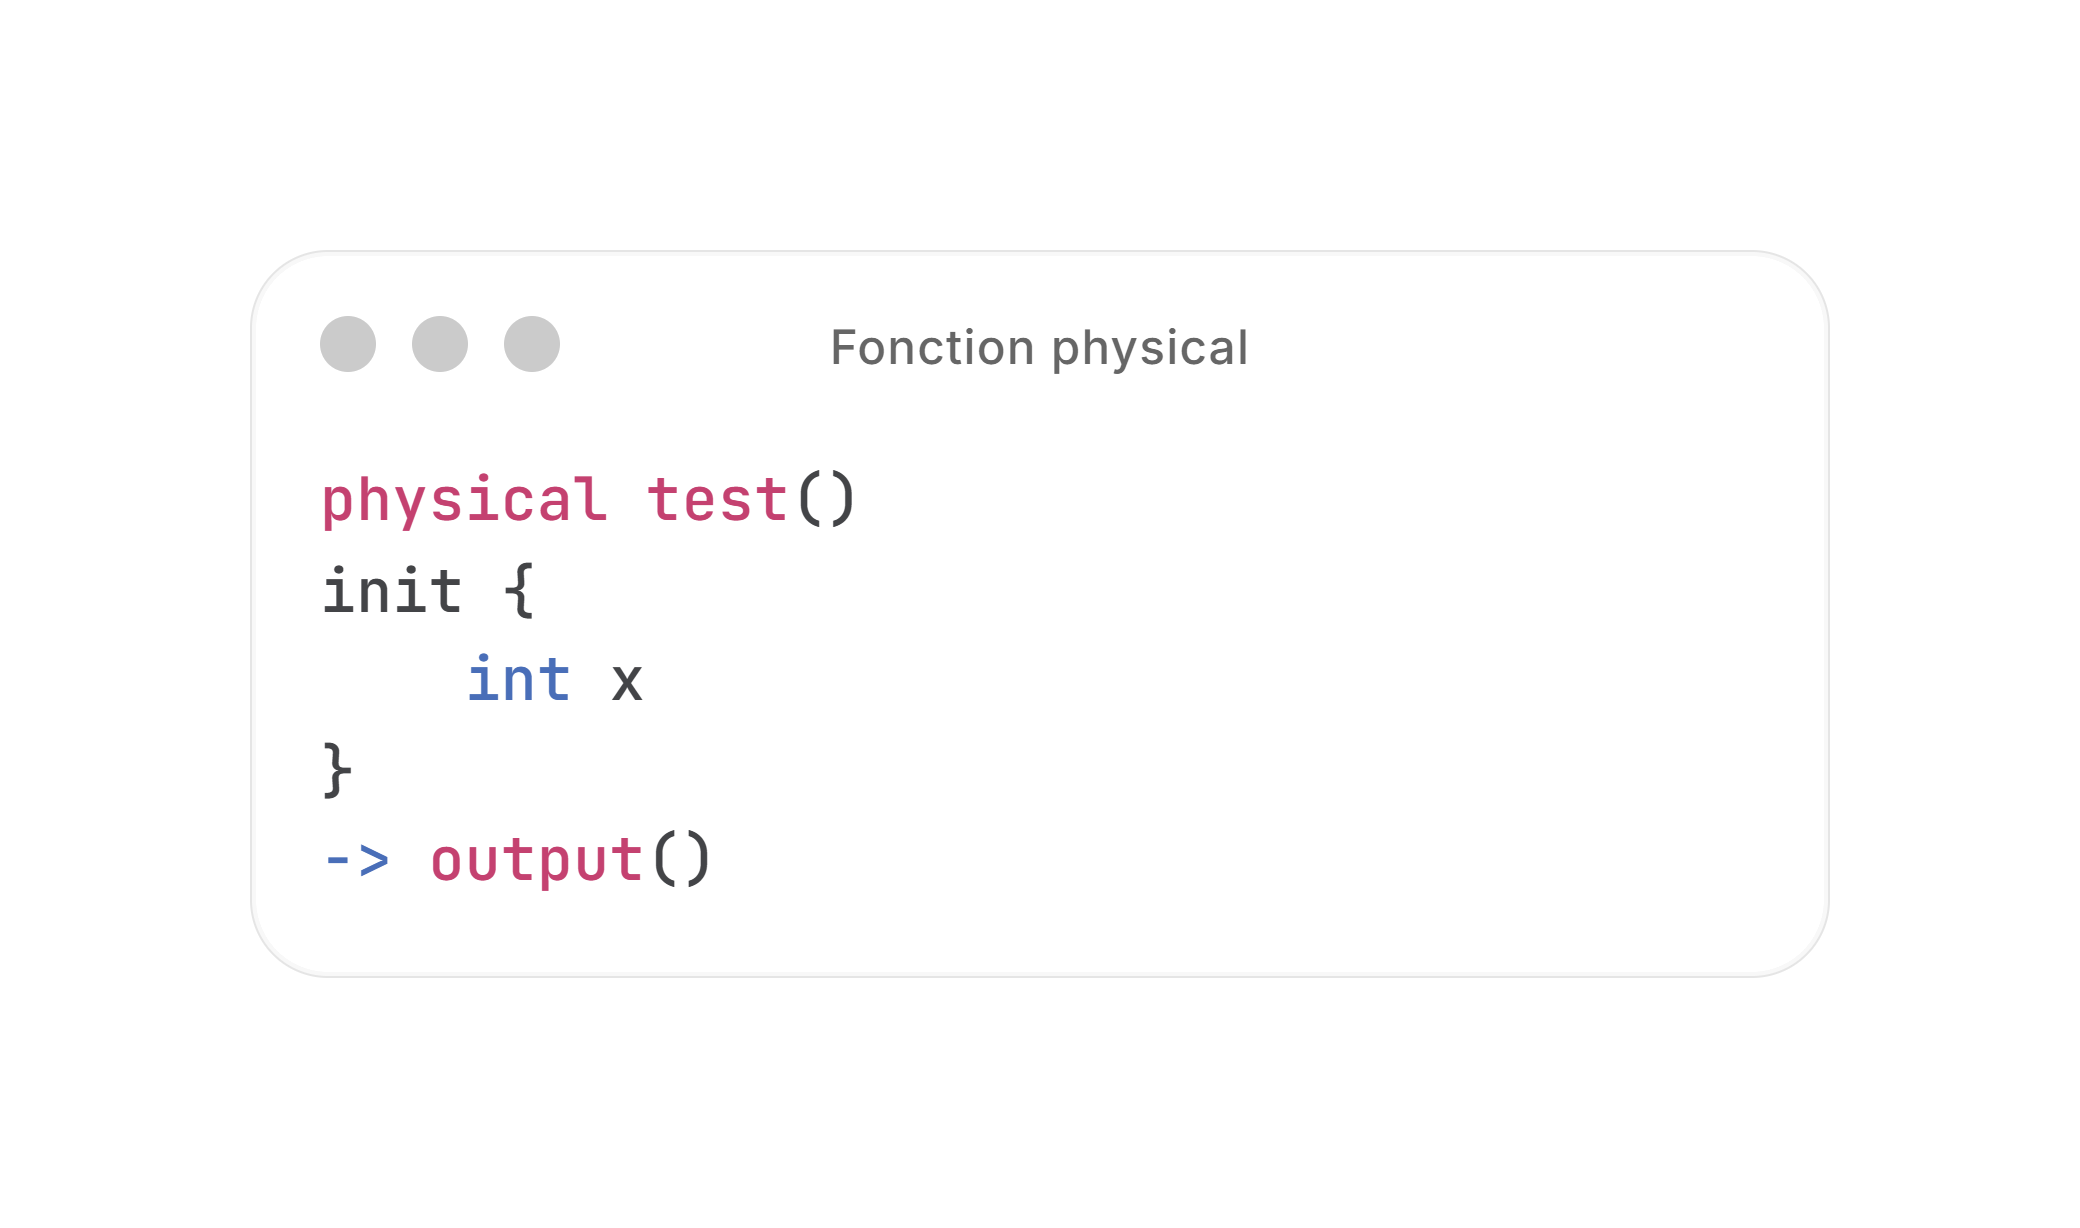
\includegraphics[width=\textwidth]{Fonction-physical.png}
    \caption{Exemple d'erreur syntaxique}
    \label{fig:erreur_syntax_physical}
\end{figure}

\begin{figure}[htbp]
    \centering
    \begin{lstlisting}[language=Chips]
x = 1 + 1.0;
    \end{lstlisting}
    \caption{Expression arithmétique CHIPS}
    \label{fig:expression_arithmetique}
\end{figure}

\begin{figure}[htbp]
    \centering
    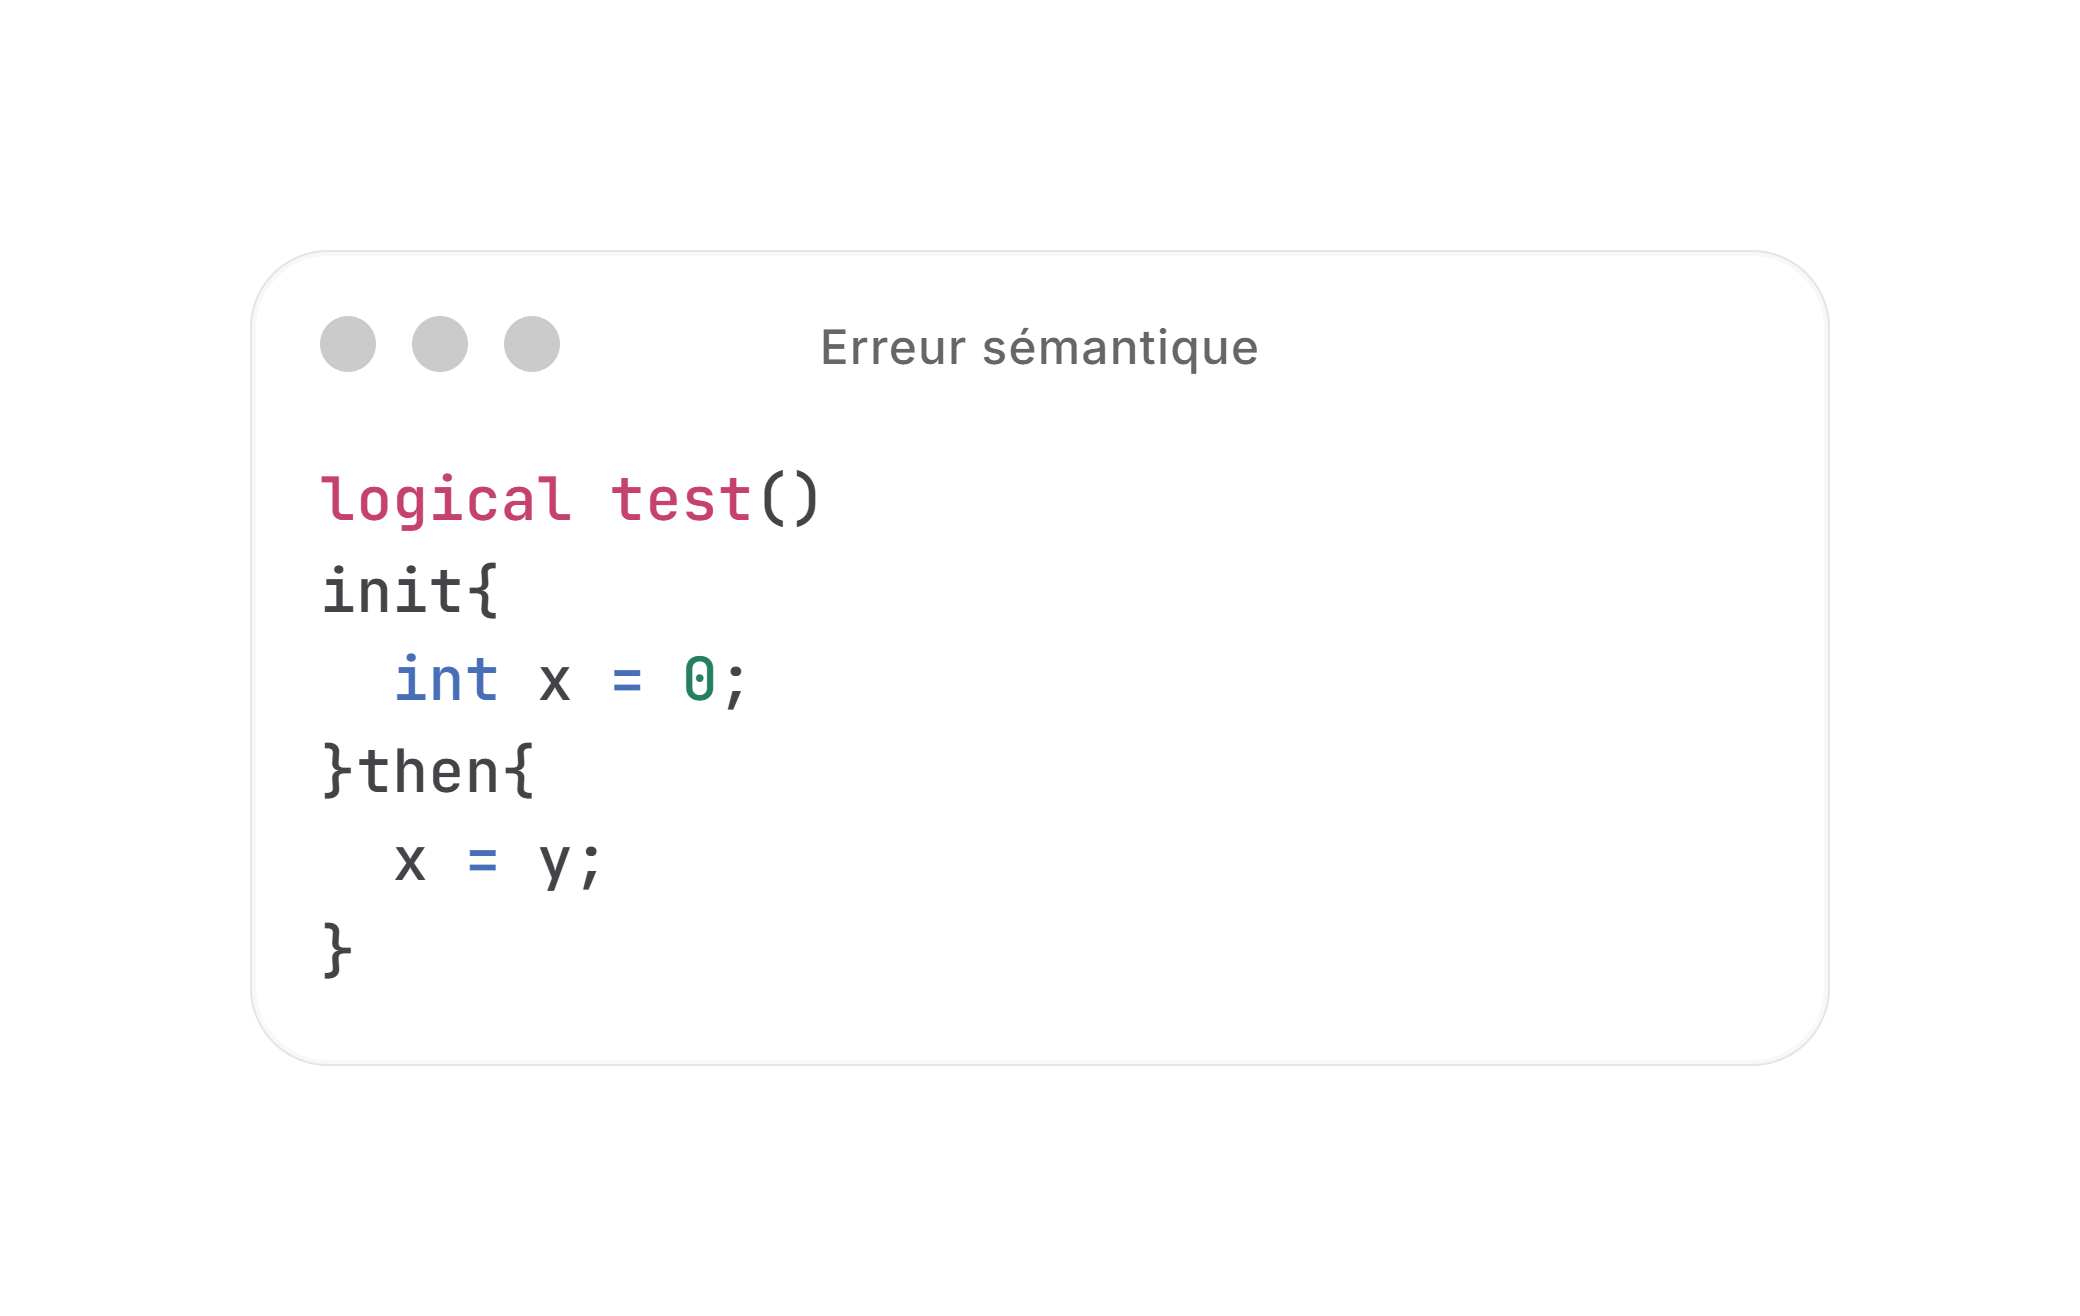
\includegraphics[width=\textwidth]{Erreur-sémantique.png}
    \caption{Exemple d'erreur sémantique}
    \label{fig:erreur_semantique}
\end{figure}

\begin{figure}[htbp]
    \centering
    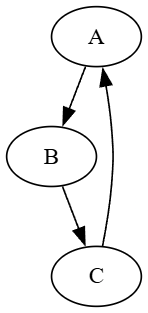
\includegraphics[width=0.6\textwidth, height=0.4\textheight, keepaspectratio]{dependance.png}
    \caption{Exemple d'erreur sur les dépendance}
    \label{fig:erreur_dependance}
\end{figure}

\newpage

\section{Tableaux}
\label{sec:tableaux}

\begin{table}[htbp]
    \centering
    \begin{tabular}{|l|l|p{5cm}|}
        \hline
        Nom de l'erreur & Exemple & Explication \\
        \hline
        TYPE\_MISMATCH & int x = 1.0 & Une variable d'un certain type ne peut recevoir des résultats d'expressions qui ne sont que de ce type.  \\
        \hline
        IMPLICIT\_CAST & 1 + 1.0 & Les expressions entre 2 types différents sont complètement impossibles. \\
        \hline
        IMPLICIT\_CAST\_ASSIGNMENT & bool b = true \&\& 1 + 1.0 & Étant donné que pour la partie de droite, il n'est pas possible de calculer son type, alors on sous-entend qu'il y a un cast implicite pour l'assignation alors que non. \\
        \hline
    \end{tabular}
    \caption{Erreurs sur les typages}
    \label{tab:erreur_typage}
\end{table}

\begin{table}[htbp]
    \centering
    \begin{tabular}{|p{8cm}|l|p{3.5cm}|}
        \hline
        Nom de l'erreur & Exemple & Explication \\
        \hline
        UNDEFINED\_FUNCTION & \makecell{logical test() -> output() \\ system \{ tests(); \}} \footnote{Ce programme ne respecte pas la grammaire mais le plus important ici c'est de comprendre pourquoi elle ne fonctionne pas}. & On essaie d'appeler une fonction qui n'est pas définie précédemment. \\
        \hline
        DUPLICATE\_FUNCTION\_DECLARATION & \makecell{logical test() -> output() \\ logical test() -> output2()} & Ici on essaye de déclarer plusieurs fois une fonction portant le même nom \\
        \hline
        WRONG\_COUNT\_OF\_ARGUMENT & \makecell{logical test() -> output() \\ system\{ test(1); \}} & On essaye d'appeler une fonction mais en n'incluant pas le bon nom d'argument. \\
        \hline
    \end{tabular}
    \caption{Erreur sur les fonctions}
    \label{tab:erreur_fonction}
\end{table}

\begin{table}[htbp]
    \centering
    \begin{tabular}{|l|l|p{5cm}|}
    \hline
        Nom de l'erreur & Exemple & Explication  \\
        \hline
         NO\_PLUGGING\_WITH\_INPUT & \makecell{logical test()-> o(1) \\ logical test2(int x = input) \\ system\{ test2() \}} & Ici la fonction test2 attend d'avoir un lien au niveau de l'input, sauf qu'il n'y en a aucun. \\
         \hline
         NO\_PLUGGING\_WITH\_OUTPUT & \makecell{logical test()-> o(1) \\ logical test2(int x = input) \\ system\{ test.o \}} & Ici la fonction test attend d'avoir un lien au niveau de son output, sauf qu'il n'y en a aucun. \\
         \hline
    \end{tabular}
    \caption{Erreur : les fonctions pas encore gérées}
    \label{tab:erreur_fonction_non_geree}
\end{table}

\begin{table}[htbp]
    \centering
    \begin{tabular}{|l|l|p{5cm}|}
         \hline
         Nom de l'erreur & Exemple & Explication  \\
         \hline
         UNDEFINED\_VARIABLE & \makecell{logical test() \\then\{x = 1;\}->o()} & Ici, on fait appel à la variable x qui n'a jamais été définie auparavant. \\
         \hline
         \makecell{DUPLICATE\_VARIABLE\\\_DECLARATION} & \makecell{logical test()\\init\{int x;\\int x = 1;\}->o()} & Ici, le problème est qu'on essaie de redéclarer la variable x. \\
         \hline
         \makecell{DUPLICATE\_VARIABLE\\\_IN\_PARAMETER} & \makecell{logical test(int x, int x) -> o()} & Ici, le problème est que le nom de paramètre x est utilisé plusieurs fois. \\
         \hline
    \end{tabular}
    \caption{Erreurs sur les variables}
    \label{tab:erreur_variable}
\end{table}

\begin{table}[htbp]
    \centering
    \begin{tabular}{|l|l|p{5cm}|}
        \hline
        Nom de l'erreur & Exemple & Explication \\
        \hline
        \makecell{NOT\_FUNCTION\\\_FOR\_LINK\_SOURCE} & \makecell{logical test()->o\\
        system\{\\test t;\\int x;\\ link x to t;\}} & Ici, le problème est que la source du lien entre les fonctions n'en est pas une.\\ 
        \hline
        \makecell{NOT\_FUNCTION\\\_FOR\_LINK\_TARGET} & \makecell{logical test()->o\\
        system\{\\test t;\\int x;\\ link t to x;\}} & Ici, le problème est que la cible du lien entre les fonctions n'en est pas une. \\
        \hline
        \makecell{FUNCTION\_PHYSICAL\\\_CANT\_BE\_SOURCE} & \makecell{physical testP()->o()\\logical testL()->o()\\system\{\\testP p;\\testL l;\\link p to l\}} & Ici, le problème est qu'une fonction physique ne peut pas être la source d'un lien car ce n'est pas possible d'avoir quelque chose de physique à l'intérieur d'une fonction physique ou même logique.\\
        \hline
    \end{tabular}
    \caption{Erreurs sur les liens}
    \label{tab:erreur_lien}
\end{table}

\end{appendix}

\newpage
\newpage
\section{Annexe : Glossaire et Mots-clés}
\label{sec:glossaire}

Cette section définit les principaux termes techniques et acronymes utilisés tout au long de ce rapport pour faciliter la compréhension du projet.

\begin{description}[style=nextline, leftmargin=1cm]
    \item[\textbf{AST (Abstract Syntax Tree)}] 
    Représentation arborescente de la structure logique d'un code source, débarrassée des détails syntaxiques purement formels (parenthèses, points-virgules).
    
    \item[\textbf{BIP (Behavior, Interaction, Priority)}] 
    Un framework de modélisation formelle vers lequel le langage CHIPS a pour vocation d'être compilé afin de permettre la simulation de systèmes temps-réel.
    
    \item[\textbf{CHIPS (Control of Hierarchical Interconnected Programmable Systems)}] 
    Langage de modélisation permettant de séparer la vue fonctionnelle d'un système de sa topologie physique.
    
    \item[\textbf{EMF (Eclipse Modeling Framework)}] 
    Framework de modélisation Java et installation de génération de code pour construire des outils et des applications basés sur un modèle de données structuré.
    
    \item[\textbf{GBT (Grammar-Based Testing)}] 
    Technique de test logiciel consistant à générer automatiquement des cas de test (fichiers .chips) en suivant les règles de production de la grammaire pour vérifier la robustesse du parseur.
    
    \item[\textbf{MDE (Model-Driven Engineering)}] 
    Ingénierie Dirigée par les Modèles ; approche de développement logiciel focalisée sur la création et l'exploitation de modèles abstraits plutôt que sur le code pur.
    
    \item[\textbf{XMI (XML Metadata Interchange)}] 
    Standard de l'OMG basé sur XML pour l'échange de métadonnées, utilisé ici pour représenter les modèles CHIPS de manière interchangeable entre différents outils de modélisation.
\end{description}
\newpage
\thispagestyle{plain}

% \begin{center}
    \rule{\textwidth}{0.5pt}
    \vspace{0.2cm}
    
    \section*{Résumé}
    
    % \begin{abstract}
    % \textbf{Résumé :} \\
    Ce rapport présente les travaux de développement et d'amélioration du compilateur pour le langage \textbf{CHIPS} (Control of Hierarchical Interconnected Programmable Systems), un langage dédié à la modélisation formelle de systèmes distribués complexes. L'objectif principal a été d'étendre les capacités du parseur existant (Flex/Bison) pour intégrer de nouvelles constructions syntaxiques, notamment les fonctions collectives (\textit{spread} et \textit{collect}). Nous détaillons la mise en place d'une chaîne de sérialisation de l'arbre de syntaxe abstraite (\textbf{AST}) vers le format \textbf{XMI}, permettant l'interopérabilité avec l'écosystème \textbf{EMF}. La fiabilité de l'outil est assurée par une gestion rigoureuse des erreurs sémantiques et par une campagne de tests automatisée s'appuyant sur le \textbf{Grammar Based Testing} (GBT).
    % \end{abstract}
    
    \paragraph{\textbf{Mots clés :}} CHIPS, C++, Grammar Based Testing, XMI, Flex, Bison/Yacc

    \vspace{1cm}

    \section*{Abstract}
    % \begin{abstract}
    \selectlanguage{english}
    % \textbf{Abstract:} \\
    This report details the development and enhancement of the compiler for the \textbf{CHIPS} language (Control of Hierarchical Interconnected Programmable Systems), designed for the formal modeling of complex distributed systems. The primary focus was extending the existing parser (Flex/Bison) to support new syntactic constructs, specifically collective functions (\textit{spread} and \textit{collect}). We describe the implementation of a serialization pipeline from the Abstract Syntax Tree (\textbf{AST}) to the \textbf{XMI} format, ensuring interoperability with the \textbf{EMF} ecosystem. Tool reliability is guaranteed through comprehensive semantic error handling and an automated testing campaign based on \textbf{Grammar Based Testing} (GBT).
    % \end{abstract}
    
    \paragraph{\textbf{Keywords :}} CHIPS, C++, Grammar Based Testing, XMI, Flex, Bison/Yacc
    
    \selectlanguage{french}
    
    \vspace{0.2cm}
    \rule{\textwidth}{0.5pt}
% \end{center}

\end{document}